\chapter{Conception et évaluation du moteur intelligent}
\label{chap:moteur-intelligent}
\newpage

\section*{Introduction}
\addcontentsline{toc}{section}{Introduction}

Le moteur de rapprochement de JobTest relie un CV et une offre à une recommandation exploitable par un recruteur. Il ne prédit ni une embauche ni une décision autonome~: il mesure une compatibilité textuelle et métier, la calibre, puis applique des règles explicites. Ce chapitre décrit les composants réellement implémentés et leur évaluation quantitative reproductible sur le corpus synthétique du projet.

\section{Objectifs et principes de conception}

Le moteur doit accepter des CV hétérogènes, confronter vocabulaire et sens général, signaler les compétences manquantes et rendre le résultat vérifiable. Le choix retenu est une fusion tardive~: chaque composant conserve son score avant agrégation. Deux couches sont séparées. La couche~1 produit le score, la décision et les justifications déterministes. La couche~2, optionnelle, enrichit seulement l'affichage par une analyse locale~; elle ne modifie ni score ni décision.

La figure~\ref{fig:chap4-pipeline} résume cet enchaînement et la place qu'y occupe la couche optionnelle.

\begin{figure}[htbp]
  \centering
  \resizebox{\textwidth}{!}{%
  \begin{tikzpicture}[node distance=7mm and 8mm,every node/.style={font=\small,align=center},>=Latex]
    \node[draw,rounded corners,fill=gray!12,minimum width=23mm,minimum height=11mm] (cv) {CV + offre\\PDF/DOCX/TXT};
    \node[draw,rounded corners,fill=gray!12,minimum width=25mm,minimum height=11mm,right=of cv] (parse) {Extraction et\\segmentation};
    \node[draw,rounded corners,fill=gray!12,minimum width=26mm,minimum height=11mm,right=of parse] (models) {TF--IDF\\embeddings\\compétences};
    \node[draw,rounded corners,fill=gray!12,minimum width=23mm,minimum height=11mm,right=of models] (fusion) {Fusion\\pondérée};
    \node[draw,rounded corners,fill=gray!12,minimum width=27mm,minimum height=11mm,right=of fusion] (decision) {Décision\\HIRE / CONSIDER / REJECT};
    \node[draw,rounded corners,fill=gray!6,minimum width=35mm,minimum height=10mm,below=of decision] (llm) {Couche~2 optionnelle~: analyse locale et questions};
    \draw[->,thick] (cv)--(parse); \draw[->,thick] (parse)--(models);
    \draw[->,thick] (models)--(fusion); \draw[->,thick] (fusion)--(decision);
    \draw[->,dashed] (decision)--(llm);
  \end{tikzpicture}
  }
  \caption{Pipeline de rapprochement de JobTest}
  \label{fig:chap4-pipeline}
\end{figure}

\section{Prétraitement et structuration des documents}

L'extraction privilégie \texttt{pdfplumber} pour les PDF et bascule sur \texttt{PyPDF2} en cas d'indisponibilité~; les fichiers DOCX sont lus avec \texttt{python-docx}, avec un repli XML. Le texte est nettoyé des URL, courriels, numéros de téléphone, retours superflus et artefacts de césure. La normalisation disponible applique, lorsque les modèles spaCy sont installés, tokenisation, lemmatisation et filtrage des mots-outils~; un repli par expressions régulières et lemmatisation légère maintient le traitement sinon.

Le CV est ensuite segmenté par intitulés français et anglais~: profil, expérience, compétences, formation, langues, certifications et projets. Cette structure n'est pas une interprétation humaine du dossier~; elle permet notamment de pondérer l'expérience distinctement des compétences.

\section{Similarité lexicale TF--IDF}

Le premier composant vectorise CV et offre avec \texttt{TfidfVectorizer}. La configuration implémentée utilise des $n$-grammes de 1 à 3 termes, au plus 10\,000 caractéristiques et une fréquence de terme sous-linéaire. TF--IDF valorise les termes discriminants~; la similarité cosinus compare les vecteurs issus des deux textes \cite{scikit_tfidf,scikit_cosine} :
\[
 \operatorname{tfidf}(t,d)=\operatorname{tf}(t,d)\log\left(\frac{N+1}{\operatorname{df}(t)+1}\right)+1,
 \qquad S_{\mathrm{TFIDF}}=\frac{\vec v_{CV}\cdot\vec v_{offre}}{\lVert\vec v_{CV}\rVert\lVert\vec v_{offre}\rVert}.
\]
Cette composante est lisible lorsque les mêmes technologies sont citées, mais elle reste sensible aux synonymes et aux reformulations.

\section{Similarité sémantique par embeddings}

Le deuxième composant encode les textes avec Sentence-Transformers lorsqu'il est disponible. Le modèle anglais configuré par défaut est \texttt{all-mpnet-base-v2}. Le modèle multilingue est identifié dans la configuration par :
\begin{center}
  \small\texttt{paraphrase-multilingual-mpnet-base-v2}
\end{center}
\texttt{HashingVectorizer} constitue le repli local en cas de chargement impossible. Les représentations de phrases et leur comparaison cosinus s'appuient sur le principe de Sentence-BERT \cite{reimers2019sbert}.

Les similitudes anglaise et multilingue sont moyennées. Une similitude par sections reçoit les poids expérience 0,40~; compétences 0,30~; résumé 0,15~; formation 0,10~; langues 0,05. Le composant retourne donc :
\[
 S_{\mathrm{emb}}=0{,}7\left(0{,}5s_{en}+0{,}5s_{multi}\right)+0{,}3s_{sections}.
\]
La pondération rend l'expérience et les compétences plus influentes sans prétendre représenter une adéquation humaine complète.

\section{Rapprochement structuré des compétences}

Le troisième composant exploite le dictionnaire versionné du projet. Il détecte les compétences techniques et comportementales, les certifications, les variantes et des $n$-grammes normalisés. Les termes de nécessité, tels que \emph{required}, \emph{must} ou \emph{obligatoire}, signalent des compétences critiques.

Soient $H$ et $S$ les recouvrements techniques et comportementaux. La base répartit les poids 0,70 et 0,30 entre les catégories présentes. Elle reçoit un bonus de domaine de 0,05, un bonus de certification plafonné à 0,10, puis une pénalité plafonnée à 0,20 pour les compétences critiques absentes :
\[
 S_{\mathrm{skill}}=\operatorname{clip}\left(S_{base}+0{,}05I_{domaine}+\min(0{,}10,0{,}03n_{cert})-0{,}20\frac{n_{critiques\ absentes}}{n_{critiques}},0,1\right).
\]
Il restitue aussi les compétences trouvées, manquantes et critiques~: ces éléments constituent la justification métier principale.

\subsection{Contrôle des preuves avant le calcul}

Un CV peut citer les compétences d'une offre sans démontrer qu'elles ont été pratiquées. Avant le calcul, la version finale applique donc trois contrôles explicables, dont le résultat accompagne chaque évaluation.
\begin{itemize}
  \item \textbf{Texte recopié de l'offre.} Toute séquence d'au moins huit mots consécutifs également présente dans l'offre est retirée du CV avant le calcul des trois composantes. Sur les 12\,000 paires du corpus, la plus longue séquence commune légitime compte sept mots~: aucune paire authentique n'est modifiée.
  \item \textbf{Mentions niées.} Une compétence citée dans une proposition négative (« aucune expérience en Kubernetes », \emph{no experience with Docker}) n'est pas comptée, et la proposition correspondante est retirée du texte utilisé pour TF--IDF et les embeddings.
  \item \textbf{Compétences déclarées ou démontrées.} Une compétence qui n'apparaît que dans une liste (section « Compétences », « Technologies » ou ligne « Skills~: \ldots ») est dite déclarée~; elle compte pour moitié dans la couverture. Une compétence citée dans l'expérience, les projets, le profil ou une certification est dite démontrée. Lorsque le CV ne comporte aucun intitulé de section reconnaissable, la distinction est impossible et toutes les mentions sont traitées comme démontrées.
\end{itemize}
Ces contrôles ne modifient aucun score des 3\,600 paires authentiques de validation et de test~; ils agissent sur les CV qui répètent l'offre ou qui reposent sur des listes déclaratives.

\section{Fusion hybride et décision}

La configuration documentée n'apprend pas les poids de fusion~; elle les fixe ainsi :
\[
 S_{hybride}=0{,}2S_{\mathrm{TFIDF}}+0{,}4S_{\mathrm{emb}}+0{,}4S_{\mathrm{skill}}.
\]
Elle donne le même poids à la proximité sémantique et à la couverture explicite des compétences. Le score brut $S_{hybride}$ reste toutefois une combinaison de similarités qui n'ont pas d'échelle commune~: la similarité cosinus de deux documents différents dépasse rarement 0,8, le recouvrement TF--IDF reste en général sous 0,5, et la fusion n'atteint pas 0,75 même lorsque chaque composante est à son maximum observé. Lu directement en pourcentage contre des bornes à 55 et 75, ce score ne produirait presque que des verdicts \texttt{REJECT}.

La version finale interpose donc une calibration versionnée entre le score brut et le score affiché. Il s'agit d'une transformation monotone, linéaire par morceaux, définie par trois points d'ancrage appris sur la partition de validation (Tableau~\ref{tab:chap4-calibration}). Elle préserve l'ordre des scores bruts jusqu'au plafond. Au-delà de 0,6126, en revanche, tous les scores affichés valent 100~: deux scores bruts distincts peuvent donc recevoir le même score affiché, et l'arrondi au dixième produit le même effet à plus petite échelle. Les AUC rapportées dans ce chapitre sont pour cette raison calculées sur les scores bruts, et le classement multi-CV départage les égalités par le score brut. La calibration laisse les sous-scores bruts inchangés dans l'explication. Chaque résultat enregistre le score brut, le score affiché, la version de calibration et les seuils appliqués.

\begin{table}[htbp]
  \centering
  \caption{Ancrages de la calibration}
  \label{tab:chap4-calibration}
  \begin{tabular}{|l|r|r|}
    \hline
    Point d'ancrage & Score brut $S_{hybride}$ & Score affiché \\
    \hline
    Origine & 0 & 0 \\
    \hline
    Frontière \texttt{REJECT}/\texttt{CONSIDER} & 0,2633 & 55 \\
    \hline
    Frontière \texttt{CONSIDER}/\texttt{HIRE} & 0,3638 & 75 \\
    \hline
    Plafond (maximum observé en validation) & 0,6126 & 100 \\
    \hline
  \end{tabular}
\end{table}

Les deux frontières sont choisies sur la validation en maximisant le macro-F1 du verdict à trois classes, comparé aux trois catégories du générateur~: paires sans rapport, profils transférables et adéquations fortes. Pour l'exemple $(S_{\mathrm{TFIDF}},S_{\mathrm{emb}},S_{\mathrm{skill}})=(0{,}10;0{,}55;0{,}20)$, le score brut vaut $0{,}32$ et le score affiché $66{,}3$. Les méthodes isolées, sélectionnables dans l'interface, disposent chacune de leurs propres ancrages.

Le \texttt{DecisionEngine} applique ensuite au score affiché les bandes du Tableau~\ref{tab:chap4-seuils}, réglables par le recruteur. Une règle de prudence complète ces bandes~: lorsque le texte recopie l'offre, ou lorsque moins de la moitié des compétences correspondantes sont démontrées, le verdict \texttt{HIRE} est remplacé par \texttt{CONSIDER}, avec une justification invitant à vérifier l'expérience. Le score affiché n'est pas modifié.

\begin{table}[htbp]
  \centering
  \caption{Bandes de décision par défaut}
  \label{tab:chap4-seuils}
  \begin{tabular}{|l|l|l|}
    \hline
    Score affiché & Recommandation & Interprétation opérationnelle \\
    \hline
    $[75,100]$ & \texttt{HIRE} & adéquation forte à examiner en priorité \\
    \hline
    $[55,75[$ & \texttt{CONSIDER} & profil à examiner avec réserves explicites \\
    \hline
    $[0,55[$ & \texttt{REJECT} & adéquation insuffisante selon les signaux disponibles \\
    \hline
  \end{tabular}
\end{table}

Ces ancrages sont appris sur des étiquettes synthétiques. Ils alignent les bandes affichées sur les classes du banc d'essai~; ils ne constituent pas une politique d'embauche validée. La confiance présentée par le moteur est une distance au seuil le plus proche, et non une probabilité d'embauche.

\section{Explicabilité et couche d'analyse locale}

La couche~1 conserve les sous-scores, poids, décision, compétences trouvées ou absentes, compétences critiques et expérience détectée. L'interface peut donc formuler une justification contrôlable, par exemple l'absence de Docker et Kubernetes parmi les prérequis.

Après ce résultat, l'interface peut demander une analyse approfondie. Le service transmet alors le texte source et ce contexte déterministe à un modèle local configuré par défaut comme \texttt{qwen2.5:1.5b}, exécuté via Ollama. La réponse structurée propose trajectoire, alertes, justification, recommandations et questions d'entretien. Les états \texttt{disabled}, \texttt{unavailable}, \texttt{error} et \texttt{inconsistent} sont contrôlés sans bloquer la couche~1~; une incohérence générative ne révise donc jamais la recommandation.

\subsection{Construction du contexte et format de réponse}

L'appel au modèle local n'est pas une requête libre. Le service assemble un contexte à partir du résultat déjà persistant~: score calibré global, sous-scores des trois composantes, décision retenue et libellé de sa bande, compétences trouvées, compétences absentes et compétences critiques manquantes. Le modèle reçoit donc le verdict comme une donnée d'entrée à commenter, et non comme une question à trancher. Le texte du CV et celui de l'offre accompagnent ce contexte pour que l'analyse puisse s'appuyer sur le contenu réel du dossier.

La réponse attendue est un objet structuré comportant cinq parties~: une lecture de la trajectoire professionnelle, les points d'attention, une justification du positionnement, des recommandations et des questions d'entretien. Cette contrainte de format sert deux objectifs. Elle rend la réponse exploitable par l'interface sans analyse de texte libre, et elle interdit au modèle de produire un score concurrent~: aucun champ ne prévoit de note chiffrée ni de verdict. Une réponse qui ne se conforme pas au schéma attendu est rejetée plutôt que corrigée, et l'état correspondant est remonté à l'interface.

\subsection{Garde-fou de cohérence et tentative d'injection}

La contrainte de format ne suffit pas. Un petit modèle exécuté sur processeur peut respecter la structure demandée tout en énonçant une appréciation qui contredit la décision statistique~: décrire comme un excellent profil un dossier que le moteur a classé en \texttt{REJECT} avec des compétences critiques absentes. Une telle réponse n'est pas seulement inexacte, elle est trompeuse, puisqu'elle apparaît à côté du verdict qu'elle dément.

Le service applique donc un contrôle de cohérence sur les cas de faible adéquation. Le texte produit est examiné à la recherche d'affirmations positives incompatibles avec le verdict, en tenant compte des négations pour éviter de sanctionner une formulation telle que « ce n'est pas un profil adapté ». Lorsqu'une contradiction est détectée, le service relance une fois le modèle avec un rappel explicite du verdict à respecter. Si la seconde réponse contredit encore la décision, l'analyse est abandonnée et l'état \texttt{inconsistent} est retourné~: le système préfère ne rien afficher plutôt qu'afficher un commentaire qui affaiblirait la recommandation. C'est un comportement de défaillance fermée, cohérent avec le principe selon lequel la couche~2 ne peut jamais réviser la couche~1.

Ce garde-fou joue également un rôle de sécurité. Le texte d'un CV est fourni par un tiers et se retrouve intégré au message envoyé au modèle~; un candidat averti pourrait y insérer des instructions destinées à l'influencer, par exemple une consigne affirmant qu'il s'agit d'un profil parfait et qu'aucune réserve ne doit être émise. L'audit de sécurité du projet a retenu ce scénario comme un risque réel. Deux propriétés le contiennent. D'une part, le score et la décision sont calculés par le moteur déterministe avant tout appel au modèle~: une injection réussie ne peut pas modifier le verdict, seulement le commentaire qui l'accompagne. D'autre part, c'est précisément sur les dossiers faiblement classés qu'une injection aurait un intérêt, et c'est là que le contrôle de cohérence est actif~: un texte trop favorable sur un dossier rejeté conduit au rejet de l'analyse. La protection n'est pas absolue, mais la surface exposée se limite à du texte consultatif, jamais à la recommandation elle-même.

\section{Jeu de données et protocole expérimental}

L'évaluation utilise \texttt{cv\_job\_dataset.csv}, généré localement avec la graine 42. Il contient 12\,000 paires CV--offre synthétiques, plusieurs domaines et niveaux d'expérience, des textes français et anglais, des abréviations, fautes de frappe, compétences obsolètes et offres contradictoires. Les étiquettes positives regroupent les cas de forte et de transférable adéquation générés~; elles ne sont pas des décisions de recrutement observées.

\subsection{Pourquoi un corpus synthétique}

Le choix d'évaluer le moteur sur des documents générés plutôt que sur de vraies candidatures mérite d'être justifié, car il conditionne la portée de tous les chiffres qui suivent. Cinq raisons l'ont motivé.

La première est l'absence de corpus disponible. Aucun ensemble de CV réels appariés à des offres, en nombre suffisant et en accès autorisé, n'a pu être réuni dans le cadre de ce stage. Les quelques dossiers accessibles se comptaient en dizaines, ce qui n'aurait permis ni un partitionnement en trois sous-ensembles, ni une mesure stable~: sur un échantillon aussi réduit, un écart de quelques paires suffit à déplacer un F1 de plusieurs points, et la comparaison entre quatre méthodes n'aurait plus été interprétable.

La deuxième raison est juridique et éthique. Un CV réel est une donnée à caractère personnel, et son usage dans un travail académique suppose une base légale, une information des personnes et une durée de conservation définie, comme le rappelle la section consacrée à ce sujet au chapitre~\ref{chap:tests-securite}. Construire un corpus de test à partir de candidatures authentiques aurait demandé des démarches que le cadre du projet ne permettait pas, et aurait introduit dans le dépôt des données qu'il aurait fallu ensuite protéger, anonymiser puis supprimer.

La troisième tient à la qualité d'extraction. Les CV réels circulent dans des formats hétérogènes, parfois exportés depuis un traitement de texte, parfois scannés, souvent mis en page sur plusieurs colonnes ou dans des tableaux. L'extraction de texte y échoue partiellement~: ordre de lecture inversé, colonnes fusionnées, caractères manquants, sections illisibles. Un échec de ce type se répercute sur les trois composantes du score. En travaillant sur des documents dont le contenu textuel est maîtrisé, l'évaluation mesure le rapprochement lui-même et non la qualité variable d'une chaîne d'extraction, dont le comportement est vérifié séparément par les tests de \texttt{parsing}.

La quatrième raison est l'absence de vérité de terrain exploitable. Même avec des CV réels, il aurait fallu disposer, pour chaque paire, d'un jugement fiable indiquant si le profil convient à l'offre. Ce jugement n'existe pas dans un dossier de candidature~: une embauche dépend d'entretiens, de disponibilités et d'arbitrages qui ne figurent nulle part dans le document. Il aurait donc fallu faire annoter des milliers de paires par des recruteurs, ce qui dépassait largement le périmètre du stage. Le générateur, lui, connaît par construction la raison pour laquelle une paire est compatible ou non, ce qui fournit une étiquette cohérente avec le critère évalué.

La cinquième est la reproductibilité. Le corpus est produit par un script du dépôt avec une graine fixée à 42~: n'importe quel lecteur peut le régénérer à l'identique, relancer le banc d'essai et retrouver les valeurs du Tableau~\ref{tab:chap4-resultats}. Un jeu de CV réels, même anonymisé, n'aurait pas pu être distribué avec le code.

J'ai écrit le générateur pour ne pas produire des documents trop faciles. Chaque CV est assemblé à partir du dictionnaire de compétences du projet, avec un domaine et un niveau d'expérience, puis dégradé volontairement~: abréviations, fautes de frappe, technologies obsolètes, formulations en français ou en anglais. Des paires contradictoires sont également générées, où le vocabulaire se recoupe alors que le profil ne correspond pas, précisément pour empêcher qu'un simple recouvrement de mots suffise. La figure~\ref{fig:chap4-exemple-cv} montre l'un de ces documents.

\begin{figure}[H]
  \centering
  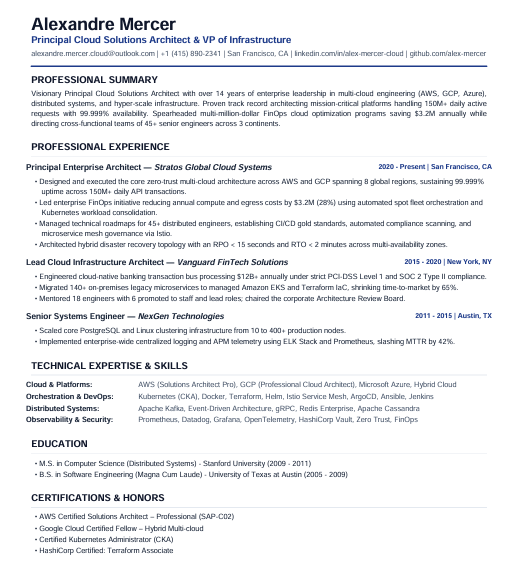
\includegraphics[width=.55\textwidth]{img/ai/example_cv.png}
  \caption{Exemple de CV synthétique}
  \label{fig:chap4-exemple-cv}
\end{figure}

Il faut néanmoins nommer ce que ce choix coûte, et le chapitre y revient dans sa section consacrée aux limites. Un document généré reste plus régulier qu'une candidature authentique~: la longueur varie peu, la structure est constante, le vocabulaire provient d'un dictionnaire fini et aucune trajectoire atypique n'y figure. Les résultats obtenus mesurent donc la capacité du moteur à distinguer des profils sur un matériau contrôlé~; ils ne préjugent pas de son comportement sur des CV réels, dont la validation reste la première étape à mener avant tout usage opérationnel.

\subsection{Partitionnement et métriques}

La séparation est stratifiée par étiquette et domaine, puis vérifiée par groupe de paire CV--offre normalisée~: 8\,400 paires pour l'apprentissage, 1\,800 pour la validation et 1\,800 pour le test final. Les poids de fusion sont fixés avant l'évaluation, le vocabulaire TF--IDF est appris sur l'apprentissage seul, les seuils binaires de chaque méthode sont sélectionnés sur la validation en maximisant le F1, et les ancrages de calibration le sont en maximisant le macro-F1 à trois classes. Les métriques sont ensuite calculées sur le test isolé. Je n'ai choisi aucun poids, seuil ni ancrage sur le test. J'ai toutefois consulté ce test à plusieurs reprises au cours du projet~: les chiffres finaux n'ont pas été réglés sur lui, mais il n'est plus strictement neuf, ce qui laisse un risque résiduel d'optimisme. Une alerte automatique signale toute méthode qui présenterait une AUC élevée et un F1 quasi nul, symptôme d'un seuil mal placé. Le partitionnement réduit la fuite de paires identiques, sans remplacer une validation externe réelle.

Les métriques sont l'exactitude, la précision, le rappel, le F1, l'AUC-ROC, l'aire précision--rappel, le kappa de Cohen et la matrice de confusion, selon les définitions de scikit-learn \cite{scikit_metrics}. Deux familles sont distinguées~: le F1 binaire, qui oppose les paires positives aux autres à un seuil donné, et le macro-F1 à trois classes, moyenne des F1 de \texttt{REJECT}, \texttt{CONSIDER} et \texttt{HIRE}, qui évalue les verdicts affichés. Ces deux mesures ne sont pas comparables entre elles. Le F1 équilibre précision et rappel :
\[
 F1=2\frac{\mathrm{precision}\times\mathrm{rappel}}{\mathrm{precision}+\mathrm{rappel}}.
\]

\section{Résultats et analyse comparative}

Le Tableau~\ref{tab:chap4-resultats} reproduit les résultats enregistrés sur les 1\,800 paires de test. Les seuils affichés sont des points de fonctionnement expérimentaux et non les seuils \texttt{HIRE}/\texttt{CONSIDER}/\texttt{REJECT} de l'interface.

\begin{table}[htbp]
  \centering
  \small
  \caption{Qualité du score brut (F1 binaire)}
  \label{tab:chap4-resultats}
  \begin{tabular}{|l|r|r|r|r|r|r|}
    \hline
    Méthode & Seuil & Exact. & Préc. & Rappel & F1 & AUC-ROC \\
    \hline
    TF--IDF & 0,04 & 0,93 & 0,93 & 0,97 & 0,95 & 0,98 \\
\hline
    Embeddings & 0,54 & 0,78 & 0,81 & 0,89 & 0,85 & 0,81 \\
\hline
    Compétences & 0,00 & 0,89 & 0,89 & 0,97 & 0,93 & 0,95 \\
\hline
    Hybride & 0,26 & 0,91 & 0,94 & 0,93 & 0,93 & 0,96 \\
    \hline
  \end{tabular}
\end{table}

La figure~\ref{fig:chap4-roc} présente les courbes ROC des scores bruts sur les mêmes paires. Elles mesurent la qualité du classement indépendamment de tout seuil~: l'AUC de la fusion (0,964) reste inférieure à celle de TF--IDF (0,979), et les embeddings seuls classent nettement moins bien (0,811). Ces courbes ne disent rien des verdicts affichés, évalués plus loin.

\begin{figure}[htbp]
  \centering
  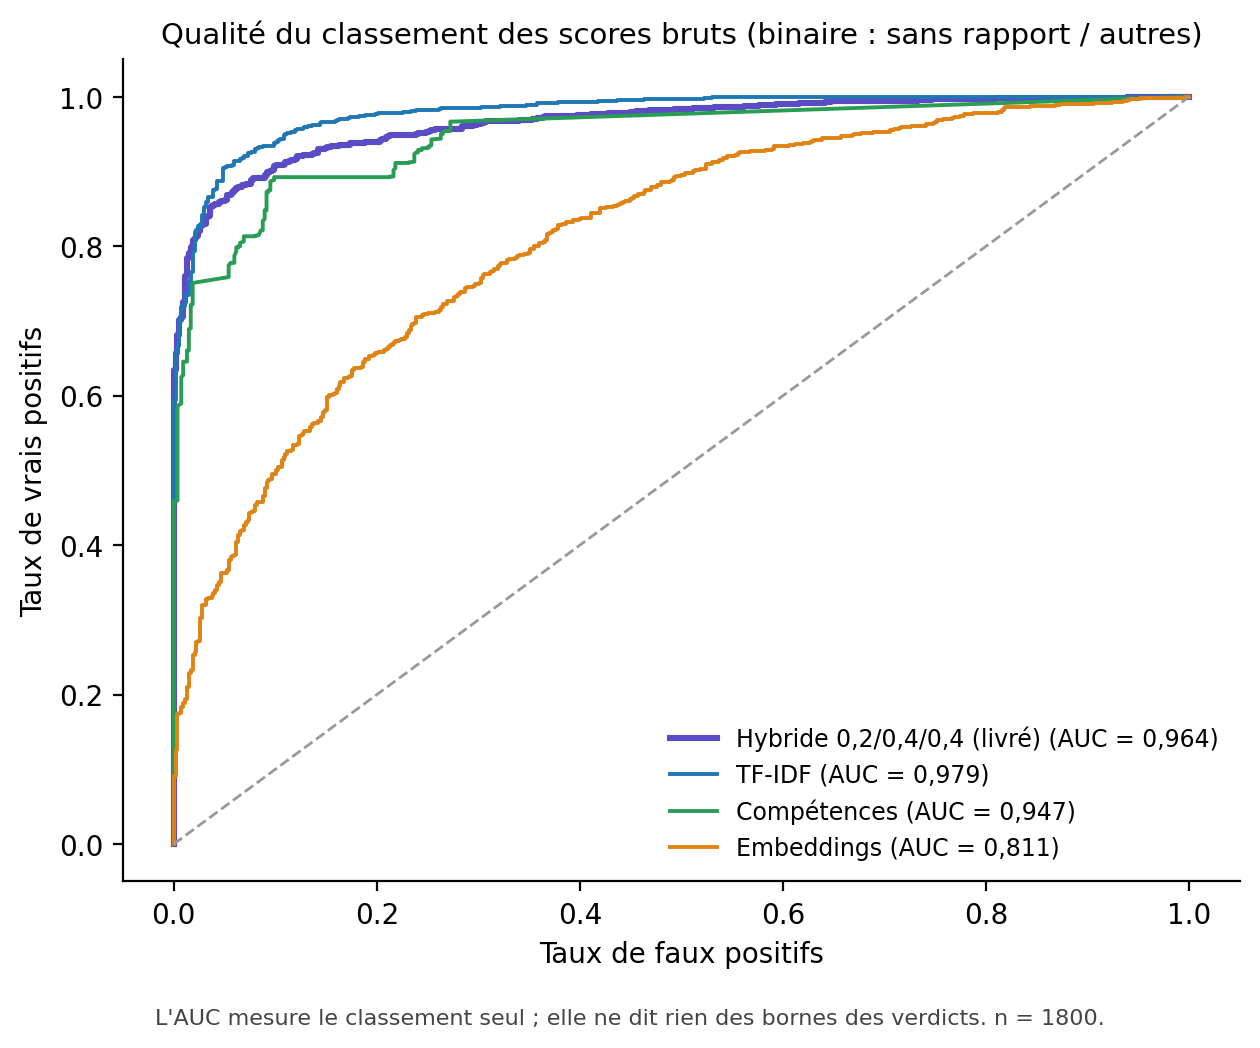
\includegraphics[width=.72\textwidth]{img/ai/eval_roc_raw.png}
  \caption{Courbes ROC des scores bruts}
  \label{fig:chap4-roc}
\end{figure}

La figure~\ref{fig:chap4-brut-classes} relie le score brut de la fusion aux trois classes synthétiques et aux deux ancrages de la calibration, qui deviennent 55 et 75 sur l'échelle affichée. Les paires sans rapport se concentrent sous le premier ancrage et la plupart des adéquations fortes au-dessus du second. Les profils transférables chevauchent les deux autres classes, ce qui annonce la difficulté de la classe intermédiaire.

\begin{figure}[htbp]
  \centering
  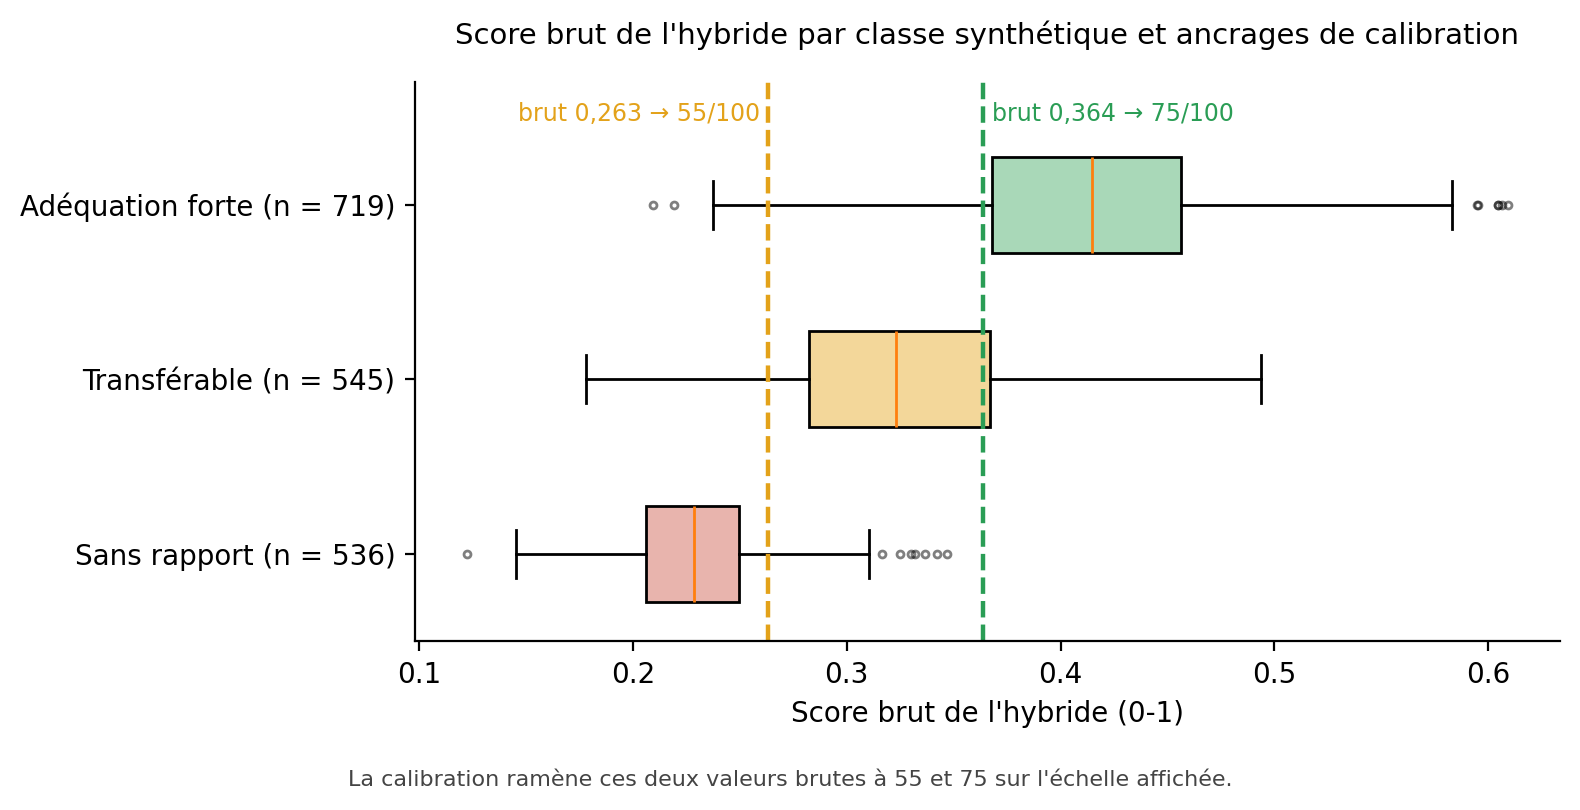
\includegraphics[width=.9\textwidth]{img/ai/eval_hybrid_raw_by_class.png}
  \caption{Score brut de la fusion par classe}
  \label{fig:chap4-brut-classes}
\end{figure}

TF--IDF obtient le meilleur F1 dans ce protocole~: $F1=0{,}95$ (intervalle bootstrap à 95~\%~: 0,941--0,959), contre $F1=0{,}93$ (0,924--0,944) et $AUC=0{,}96$ pour la fusion. Sur les mêmes 1\,800 paires, chacune lue à son propre seuil de validation, TF--IDF classe correctement 108 paires que la fusion manque, et l'inverse se produit pour 73 paires~; le test de McNemar donne $p\approx0{,}011$. Ce protocole ne permet donc pas de revendiquer une supériorité mesurée de l'hybride~: la différence observée va dans le sens inverse. Elle ne démontre pas pour autant une supériorité générale du lexical, car le générateur construit CV et offres à partir d'un vocabulaire contrôlé et partagé, ce qui favorise le recouvrement des termes. La fusion est retenue pour des raisons que ce benchmark ne mesure pas~: la justification par compétences restituée au recruteur et une moindre sensibilité à la reformulation, observée sur l'expérience contrôlée du Tableau~\ref{tab:chap4-bug4}. Le temps moyen mesuré est 55,85~ms par paire pour la fusion, contre 921,60~ms pour les embeddings seuls dans cet environnement.

\subsection*{Verdicts affichés par la version finale}
\addcontentsline{toc}{subsection}{Verdicts affichés par la version finale}

Le Tableau~\ref{tab:chap4-resultats} mesure la capacité de discrimination du score brut. Le Tableau~\ref{tab:chap4-verdicts} évalue ce que voit le recruteur, c'est-à-dire les verdicts \texttt{REJECT}, \texttt{CONSIDER} et \texttt{HIRE}, sur les mêmes 1\,800 paires de test. Celles-ci comptent 536 paires sans rapport, 545 profils transférables et 719 adéquations fortes.

\begin{table}[H]
  \centering
  \footnotesize
  \caption{Qualité des verdicts affichés}
  \label{tab:chap4-verdicts}
  \begin{tabular}{|>{\raggedright\arraybackslash}p{3.7cm}|>{\centering\arraybackslash}p{2.5cm}|>{\centering\arraybackslash}p{1.2cm}|>{\centering\arraybackslash}p{1.7cm}|>{\centering\arraybackslash}p{1.1cm}|>{\centering\arraybackslash}p{2.3cm}|}
    \hline
    Configuration & Macro-F1 3 classes [IC 95~\%] & F1 \texttt{HIRE} & F1 binaire \texttt{CONSIDER} ou mieux & Kappa q. & Verdicts R / C / H \\
    \hline
    \textbf{Hybride calibré (version finale)} & \textbf{0,740} [0,720--0,760] & 0,782 & 0,934 & 0,799 & 548 / 557 / 695 \\
    \hline
    TF--IDF seul, calibré & 0,746 [0,726--0,765] & 0,758 & 0,950 & 0,797 & 471 / 641 / 688 \\
    \hline
    Fusion apprise 0,75 / 0,05 / 0,20, calibrée (non retenue) & 0,780 [0,761--0,799] & 0,792 & 0,957 & 0,833 & 552 / 560 / 688 \\
    \hline
  \end{tabular}
\end{table}

La figure~\ref{fig:chap4-verdicts-repartition} compare la répartition des verdicts à celle des classes synthétiques. La version finale produit une répartition proche de celle des classes, sans que cette proximité suffise à garantir que chaque paire reçoive le bon verdict.

\begin{figure}[htbp]
  \centering
  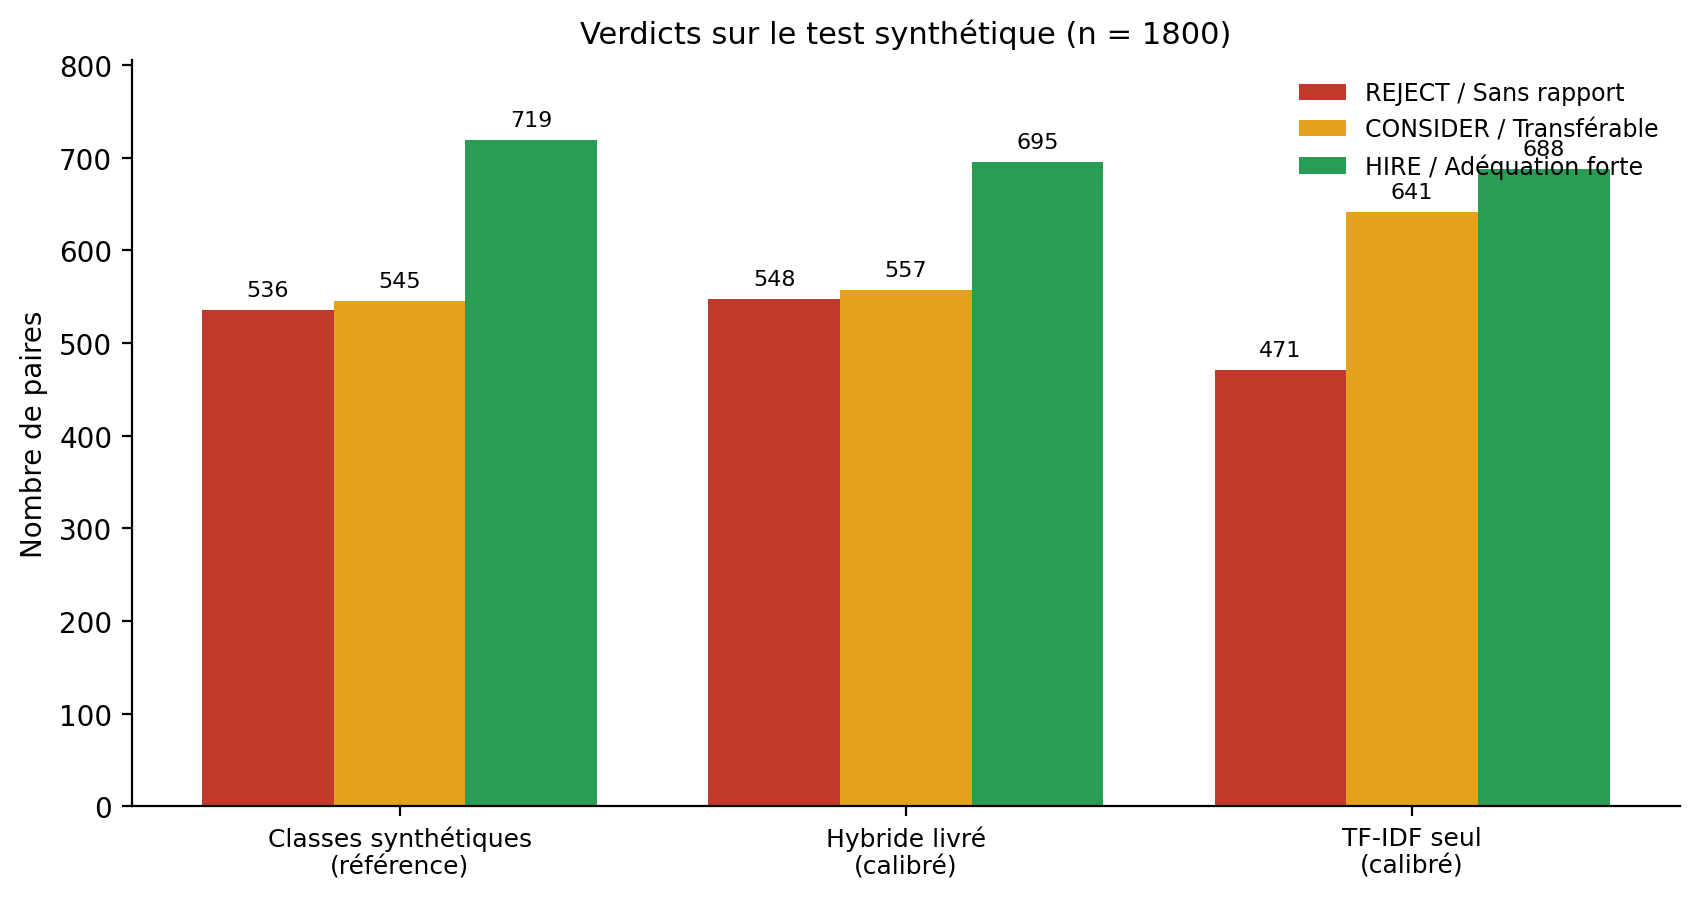
\includegraphics[width=.92\textwidth]{img/ai/eval_verdict_distribution.png}
  \caption{Répartition des verdicts}
  \label{fig:chap4-verdicts-repartition}
\end{figure}

La matrice de confusion de la version finale (figure~\ref{fig:chap4-confusion-verdicts}) montre que les erreurs se concentrent entre classes voisines. Les paires sans rapport sont bien identifiées (459 \texttt{REJECT} sur 536, aucune \texttt{HIRE}), et 553 des 719 adéquations fortes reçoivent \texttt{HIRE}. La classe intermédiaire reste la plus difficile (F1 de 0,59)~: 325 profils transférables sur 545 reçoivent \texttt{CONSIDER}, 142 \texttt{HIRE} et 78 \texttt{REJECT}. Une comparaison appariée par bootstrap sur les mêmes paires ne montre pas de différence entre l'hybride calibré et TF--IDF seul (écart de $-0{,}006$, IC à 95~\% de $-0{,}028$ à $0{,}016$). Les paires multilingues (CV anglais, offre française, 120 paires) sont moins bien traitées que les paires françaises (exactitude de 0,65 contre 0,75).

\begin{figure}[htbp]
  \centering
  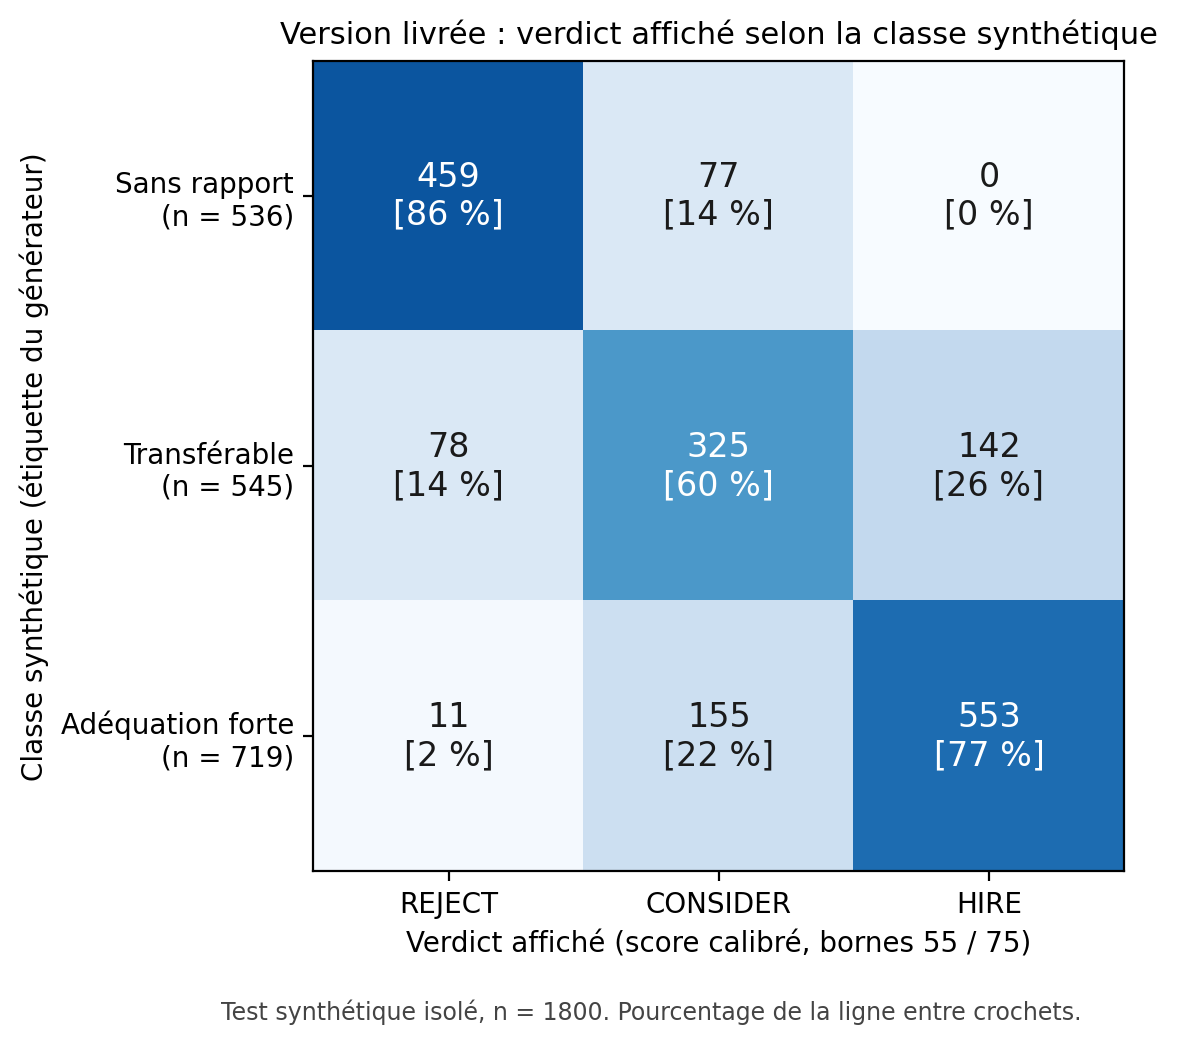
\includegraphics[width=.7\textwidth]{img/ai/eval_confusion_verdicts.png}
  \caption{Matrice de confusion des verdicts}
  \label{fig:chap4-confusion-verdicts}
\end{figure}

\subsection*{Choix de la pondération}
\addcontentsline{toc}{subsection}{Choix de la pondération}

Une fusion dont les poids sont appris sur l'apprentissage seul (0,75 / 0,05 / 0,20) obtient le meilleur macro-F1 en validation comme en test, et la règle de sélection fixée avant la lecture du test la désignait. Elle n'est pas retenue pour le produit, pour deux raisons. D'abord, son avantage provient d'un corpus dont les étiquettes sont construites à partir du recouvrement des compétences recopiées dans l'offre, ce qui favorise mécaniquement le signal lexical. Ensuite, une pondération dominée par TF--IDF récompense la simple reprise du vocabulaire de l'annonce. Sur une paire contrôlée de CV de même substance, l'un calqué sur l'offre et l'autre reformulé, une pondération 0,9 / 0,0 / 0,1 donnait un écart de 25,6 points, contre 9,6 points avec la pondération documentée (Tableau~\ref{tab:chap4-bug4}). La version finale conserve donc la pondération documentée 0,2 / 0,4 / 0,4~; la calibration de la fusion apprise est archivée avec le code.

\begin{table}[H]
  \centering
  \small
  \caption{Effet de la reformulation selon la pondération}
  \label{tab:chap4-bug4}
  \begin{tabular}{|l|r|r|r|}
    \hline
    Pondération du moteur & CV calqué sur l'offre & CV reformulé & Écart \\
    \hline
    0,9 / 0,0 / 0,1 & 99,2 & 73,6 & 25,6 points \\
    \hline
    0,2 / 0,4 / 0,4 (documentée) & 94,4 & 84,8 & 9,6 points \\
    \hline
  \end{tabular}
\end{table}

\subsection*{Robustesse face aux CV manipulés}
\addcontentsline{toc}{subsection}{Robustesse face aux CV manipulés}

Le Tableau~\ref{tab:chap4-robustesse} mesure l'effet du contrôle des preuves sur des CV de la partition de validation modifiés de façon contrôlée, à raison de 200 paires par scénario. Les cinq premiers scénarios partent de profils sans rapport avec l'offre~; les deux derniers partent d'adéquations fortes. Les deux colonnes utilisent la même calibration~; seule change la présence du contrôle des preuves. Je n'ai ajusté aucun paramètre sur ces scénarios.

\begin{table}[htbp]
  \centering
  \footnotesize
  \caption{Effet du contrôle des preuves}
  \label{tab:chap4-robustesse}
  \begin{tabular}{|p{7.2cm}|c|c|}
    \hline
    Scénario & Sans contrôle & Version finale \\
    \hline
    Référence~: profils sans rapport non modifiés & \multicolumn{2}{c|}{174 / 25 / 1} \\
    \hline
    Profil sans rapport + liste d'exigences de l'offre recopiée & 0 / 0 / 200 & 133 / 67 / 0 \\
    \hline
    Profil sans rapport + mêmes compétences, réordonnées, dans une section Compétences & 0 / 0 / 200 & 0 / 200 / 0 \\
    \hline
    Profil sans rapport + offre entière collée & 0 / 0 / 200 & 174 / 26 / 0 \\
    \hline
    Profil sans rapport + mention niée des compétences & 0 / 0 / 200 & 175 / 24 / 1 \\
    \hline
    Profil sans rapport + compétences insérées dans une phrase d'expérience & 0 / 0 / 200 & 0 / 0 / 200 \\
    \hline
    Référence~: adéquations fortes non modifiées & \multicolumn{2}{c|}{1 / 33 / 166} \\
    \hline
    Adéquation forte privée de la moitié de ses compétences & 15 / 129 / 56 & 15 / 129 / 56 \\
    \hline
    Adéquation forte allongée par des expériences sans rapport & 0 / 16 / 184 & 0 / 16 / 184 \\
    \hline
  \end{tabular}
\end{table}

Le contrôle ramène les listes recopiées, l'offre collée et les mentions niées au niveau de la référence non modifiée~: aucun CV à liste recopiée ou à offre collée n'obtient \texttt{HIRE}, et le seul \texttt{HIRE} restant parmi les mentions niées correspond à un profil déjà mal classé avant modification. Une liste réordonnée placée dans une section Compétences n'est pas reconnue comme copie, mais la règle de prudence ramène le verdict à \texttt{CONSIDER}. Les CV partiels et les CV longs ne sont pas affectés, et aucun verdict des 1\,800 paires authentiques de validation ne change. En revanche, un CV qui affirme une expérience dans une phrase rédigée reste classé \texttt{HIRE}~: l'analyse du texte ne peut pas distinguer une déclaration mensongère d'une expérience réelle. Cette limite justifie la lecture humaine du dossier et les questions d'entretien proposées par la couche~2.

Sur le déploiement Azure CPU, un essai de couche~2 a produit les cinq sections attendues en 54\,290,6~ms. Cette mesure ponctuelle décrit la démonstration, non une garantie de latence ou une évaluation de qualité générative.

\section{Limites, risques et perspectives}

Les résultats quantitatifs sont internes à un corpus synthétique et à des étiquettes générées par règles~; les ancrages de calibration sont appris sur ces étiquettes. Les essais que j'ai menés avec mes propres CV face à des offres réelles, présentés au chapitre~\ref{chap:tests-securite}, sont fonctionnels~: faute de jugements de référence établis par des recruteurs, ils ne permettent de calculer ni précision, ni rappel, ni F1. Les mesures ne couvrent ni la qualité d'une embauche, ni les effets sur les candidats, ni l'équité entre groupes protégés. Un CV qui décrit faussement une expérience n'est pas détecté. Le dictionnaire peut omettre une technologie ou mal qualifier un intitulé ambigu~; les embeddings peuvent rapprocher des contenus trop généraux~; le modèle local peut produire une justification plausible mais erronée. JobTest doit donc rester une aide à la priorisation, avec révision humaine, traçabilité des critères et possibilité de correction.

Les suites nécessaires sont une validation avec des recruteurs sur des données autorisées et minimisées, la mesure de l'accord inter-évaluateurs, des tests de biais et de robustesse par sous-groupes, ainsi qu'un réapprentissage des ancrages de calibration sur ces données annotées. L'évaluation du modèle de langage doit être séparée de celle du score~: fidélité aux faits, utilité des questions et taux d'incohérences sont des axes distincts.

Le tableau~\ref{tab:chap4-synthese} récapitule le rôle de chaque couche et le garde-fou qui lui est associé.

\begin{table}[H]
  \centering
  \caption{Synthèse des couches}
  \label{tab:chap4-synthese}
  \begin{tabular}{|p{3cm}|p{4cm}|p{5cm}|}
    \hline
    Couche & Rôle & Statut et garde-fou \\
    \hline
    Couche~1 & score hybride calibré, contrôle des preuves, décision et explications & implémentée~; décision déterministe~; \texttt{HIRE} écarté si les preuves sont insuffisantes \\
\hline
    Couche~2 & analyse locale et questions d'entretien & optionnelle~; ne change jamais la couche~1 \\
\hline
    Évaluation & benchmark train/validation/test synthétique & disponible~; ancrages appris sur étiquettes synthétiques~; non représentatif d'une embauche réelle \\
    \hline
  \end{tabular}
\end{table}

\section*{Conclusion}
\addcontentsline{toc}{section}{Conclusion}

Le moteur combine signaux lexicaux, sémantiques et structurés, contrôle les preuves avant le calcul et calibre son score avant d'appliquer les bandes de décision. Sur le test synthétique, les verdicts affichés atteignent un macro-F1 de 0,740 sur trois classes, sans dépasser TF--IDF seul, et les CV qui recopient l'offre n'obtiennent plus \texttt{HIRE}. La calibration devra être réapprise sur des données réelles annotées avant tout usage opérationnel. Le chapitre suivant présente la réalisation de la plateforme.
